
\documentclass[preprint,10pt]{elsarticle}
\makeatletter
\def\ps@pprintTitle{%
 \let\@oddhead\@empty
 \let\@evenhead\@empty
 \def\@oddfoot{\centerline{\thepage}}%
 \let\@evenfoot\@oddfoot}
\makeatother
%% Use the option review to obtain double line spacing
%% \documentclass[preprint,review,12pt]{elsarticle}

%% Use the options 1p,twocolumn; 3p; 3p,twocolumn; 5p; or 5p,twocolumn
%% for a journal layout:
%% \documentclass[final,1p,times]{elsarticle}
%% \documentclass[final,1p,times,twocolumn]{elsarticle}
%% \documentclass[final,3p,times]{elsarticle}
%% \documentclass[final,3p,times,twocolumn]{elsarticle}
%% \documentclass[final,5p,times]{elsarticle}
%% \documentclass[final,5p,times,twocolumn]{elsarticle}


\usepackage{graphicx}
\usepackage{amssymb}

\usepackage[margin=2.5cm]{geometry}
\usepackage{caption}
\usepackage{subcaption}
\setlength\parindent{12pt}


\begin{document}

\begin{frontmatter}

\title{Applying Topological Methods to Gene Expression Analysis}


\author{Conrad De Peuter, BS}
\author{Vijayaraghavan Balaji, B.Tech}
\address{Columbia University, New York, NY, USA}

\begin{abstract}
Finding differentially expressed genes from cancer microarrays is a common technique used in determining the causes of cancer, but extracting meaning from this set of genes is often not straightforward. Regular clustering methods routinely group genes that are not biologically related, thus it is hard to extract information from such analyses. Using a topological data analysis method known as Mapper in conjunction with data on gene functions as well as the pathways where these genes operate, we find evidence that clusterings produced by Mapper  have more biological significance than regular clustering methods K-Means and Hierarchical Clustering. The functional clustering of these genes may provide insight for novel areas of investigation in determining the causes/prognosis for cancers.
\end{abstract}

\end{frontmatter}

\section{Introduction}
\subsection{Mapper/PAD}
The Mapper method, introduced by Carlsson et. al. in 2007 \cite{mapper} formulated a novel topological approach to analysis of high-dimensional data sets. The idea is based on partial clustering of the data combined with a filtering function on the data to reduce its dimensionality. The method performs partial clustering on overlapping intervals of the data set with a graph output where vertices are the bins within each clustering. Because the intervals are overlapping a data point may end up in multiple clusters, if this happens an edge is drawn between these two clusters in the graph. With a well defined set of filters, Carlsson et. al. were able to show that relationships among data points persisted throughout the dimensional reduction that did not persist in regular clustering algorithms. In an approach termed Progression Analysis of Disease (PAD), Nicolau et al. applied the Mapper method to breast cancer microarray data in 2011 using a filter function referred to as Disease-Specific Genomic Analysis (DSGA) \cite{dsga}, and were able to identify a type of breast with unique gene profiles, and discovered that patients with this cancer had 100\% survival rates and no metastasis  \cite{nicolau}. Previously, Mapper had been shown to provide structural insight into the folding of RNA \cite{RNA}. In this study we intend to provide further evidence of Mapper's ability to produce functionally significant clusterings. According to Carlsson et al.'s original paper on Mapper, the goal of the method is to build low-dimensional image of the data set which may indicate areas of interest. Applying this method to cancer data in a similar fashion to PAD, we would like to indicate areas of interest for studying two specific forms of cancer, as well as provide a general framework for similar studies in the future. 

\subsection{Benefits of Discovering Functionally Significant Clusters}
The possible benefits of such a technique are clear. The ability to identify a subgroup of cancers with unique and consistent survival rates not only helps with patient prognosis, it may also provide insight into treatment methods. Unlike the PAD study we do not have access to the survival rates of the patients in the data set, we only have the gene expression data from the time it was taken. In lieu of this our final goal is not to find specific high or low survival rate cancers, but instead to develop a method which produces areas of interest for further study of these cancers by examining the functions of genes which end up clustered together, as well as pathways where they operate.

\section{Methods and Materials}
\subsection{Data Sources}
We used two data sets from the Gene Expression Omnibus. GDS5437 \cite{gds5437} compares 14 lung tissue samples of gene expression of healthy mice versus mice with non-metastatic and metastatic breast cancer tumors. These samples consisted of 5 healthy mice, 5 with non-metastatic tumors, and 4 with metastatic tumors. The original study for the data set was looking at the over-expression of the G-CSF glycoprotein in the lung tissue of mice with metastatic breast cancer, and showed that in the lung tissue of these mice only those with metastatic breast cancer showed over-expression of G-CSF. We are also looking at a second data set. GDS1439 \cite{gds1439} compares 19 samples of prostate cancer tumors in humans which are benign (6), clinically localized (7), and metastatic (6). The original study for this data set looked to identify which proteins were altered in the different states of cancer and tried to identify a proteomic progression signature in prostate tumors. 


\subsection{Data Dimensioniality Reduction}
	Before clustering we reduced the number of genes in each data set in order to make hundreds of clusterings computationally feasible. We did this by removing genes which did not have a sufficient expression level across enough samples using the "genefilter" package in R \cite{genefilter}. We then fit a linear model to each of the data sets to identify which genes were differentially expressed. GDS1439 produced thousands of differentially expressed genes, so we took the ones with the top 1000 p-values. GDS5437 only produced 76 differentially expressed genes, so we took all of those. For both data sets we reduced each to around 7000 genes.
	
	The crux of the Mapper algorithm is a dimensionality reducing filter function which "reflects geometric properties of the data set" \cite{mapper}. The topological theory of the method is that if this filtering function relates to the areas of interest in the data set then the proximity of similar data points should persist through this dimensionality reduction. We used the same filter function from the PAD/DSGA method \cite{nicolau}, which isolates the diseased component of every data point/vector by removing the normal component from all points. They hypothesize that data from diseased tissue can be summarized into the following equation: $\vec{T} = Nc.\vec{T} + Dc\vec{T}$, and they would like to isolate $Dc\vec{T}$. If two genes perform a similar function in the context of a disease, then their gene expression data should remain close after this dimensionality reduction.
		
	After finding these genes and reducing the dimension we performed three types of cluster analysis on the data, using the Biological Homogeneity Index (BHI), a method introduced by Datta \& Datta in 2006 \cite{bhi}, to compare the functional significance of the clusters produced by Mapper, K-Means, and Hierarchical Clustering. To find the optimal clustering of the genes we performed a grid analysis across the parameters for Mapper: number of intervals, overlap between intervals, and number of bins to use when clustering in the intervals. Mapper also takes a point-wise distance matrix as an input, and for this we experimented with both the Pearson and Spearman metrics, finding optimal results with Pearson. For each set of parameters to Mapper we took the number of vertices in the outputted graph, and set that to k for K-Means, and cut the Hierarchical Clustering tree at the level which would produce that many clusters. By looking at the clustering which produced the optimal BHI for Mapper, which happened to be the clustering which had the highest difference in performance compared to the other two methods, we argue that the clustering produced by Mapper is more biologically significant than the other methods. To do so we continued with a more detailed analysis of the contents of the clusters.


\section{Results}


\subsection{General Mapper Comparison}
	Searching through hundreds of parameter combinations we found that for GDS1439, the BHI of Mapper's clustering was noticeably larger than that of either K-Means or Hierarchical Clustering, although not outside of a standard deviation. For the clusterings where hundreds of genes were placed in each cluster there was no noticeable difference, but once the number of clusters was past 100 the BHI's of the Mapper clusters had a noticeable improvement. This result seems somewhat intuitive if you accept the hypothesis that Mapper produces functionally significant clusters; with hundreds of genes in a single cluster there are bound to be many unrelated genes and thus a lot of noise. Once the number of genes in a single cluster is reasonably small the opportunity for a method specifically aimed at discovering functional significance to show its worth is realizable. Tables 1 \& 2 show the clusterings' BHI's, for all genes, as well as just the differentially expressed genes in each cluster. Figure 1 shows the relationship between BHI and number of clusters for each method.	
	
\begin{figure}
  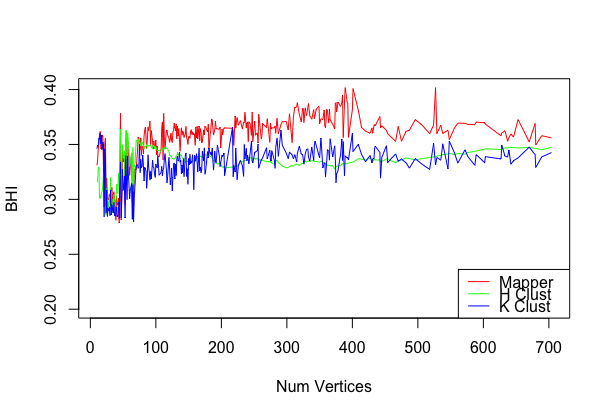
\includegraphics[width=\linewidth]{plotTrend}
  \caption{As the number of clusters rises, the BHI of Mapper clusterings separates itself}
  \label{bhi-trend}
\end{figure}

	
\begin{table}[]
\centering
\caption{BHI's for GDS1439's clusters, as well as just the differentially expressed genes within a cluster. Error bars are standard deviations for each set of output BHI's}
\label{table-bhi-1439}
\begin{tabular}{llllllll}
         & Mapper            & H-Clust           & K-Means           & Mapper-DEG        &  H-Clust-DEG        & K-Means-DEG       & Obs \\
Pearson  & $.3429 \pm .030$ & $.3275 \pm .022$ & $.3240 \pm .025$ & $ .3516 \pm .016$ & $ .3370 \pm .010 $ & $ .3300 \pm .018 $ & 759 \\
Spearman & $.3538 \pm.013$  & $.3462 \pm .012$  & $.3396 \pm .038$ & $ .3139 \pm .039$ & $ .3285 \pm .032$  & $ .3400 \pm .038 $ & 520
\end{tabular}
\end{table}

\begin{table}[]
\centering
\caption{BHI's for GDS5437}
\label{table-bhi-5437}
\begin{tabular}{llllllll}
         & Mapper            & H-Clust           & K-Means           & Mapper-DEG        & H-Clust-DEG       & K-Means-DEG       & Obs \\
Pearson  & $.3074  \pm .012$ & $.3266 \pm .017 $ & $ .2990 \pm .006$ & $ .3023 \pm .022$ & $ .3205 \pm .022$ & $ .3218 \pm .033$ & 264 \\
Spearman & $.3253 \pm .009$  & $ .3368 \pm.019 $  & $.2526 \pm .031$  & $ .2739 \pm .028$ & $ .2196 \pm .022$ & $ .2526 \pm .033$ & 550
\end{tabular}
\end{table}

While the results were promising for GDS1439, they were not for GDS5347. In the latter hierarchical clustering produced the best BHI results for complete clusters, and K-Means did best for just differentially expressed genes. While BHI is a good metric for an at-glance look at the functional significance of each clustering method we believe more analysis is necessary before we can fully argue for the benefits of Mapper. To do so we go further into our analysis of GDS1439 with three types of analysis. We found the optimal Mapper parameters of overlap, intervals, and bins, to be 26, 20, and 35, which resulted in a BHI of .402 for Mapper, and 0.332 and 0.340 for H and K Clustering respectively. After choosing these parameters we compared the functions of the genes in each cluster, the pathways where those genes operate, as well as a Gold Standard analysis of the clustering destination of genes which are known to be related to prostate cancer. 

\subsection{Gold Standard Analysis}
	To analyze the clustering we compiled a gold standard of genes known to be related to prostate cancer from the Genetics Home Reference \cite{pcgenes}. On obtaining the optimal parameter combination of overlap, intervals and bins, for which the BHI values of Mapper are significantly higher than K-means and Hierarchical clustering, we analyzed where the gold standard genes for each data set end up in each method. We believe that if gold standard genes are clustered together by Mapper, but not by the other methods, this provides strong evidence that Mapper produces clusters of functional significance. The clustering destination of our gold standard genes is show in in Figure 2.
\begin{figure}
\centering
\begin{subfigure}{.5\textwidth}
  \centering
  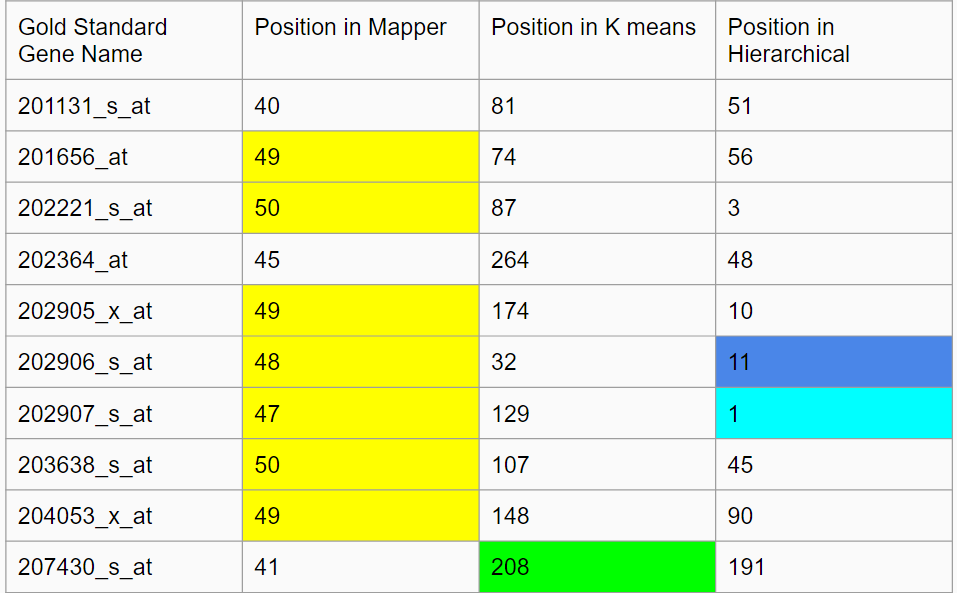
\includegraphics[width=1\linewidth]{goldstandard1.png}
  \label{fig:sub1}
\end{subfigure}%
\begin{subfigure}{.5\textwidth}
  \centering
  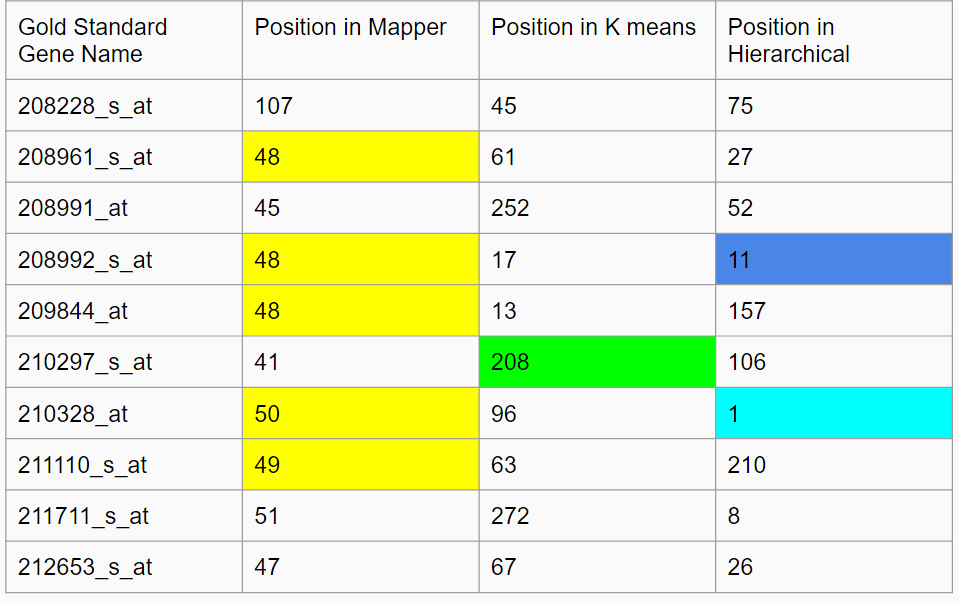
\includegraphics[width=1\linewidth]{goldstandard2.png}
  \label{fig:sub2}
\end{subfigure}
\caption{The clustering destination of each of our gold standard genes for each method.}
\label{fig:test}
\end{figure}

On performing clustering analysis of the Gold Standard genes, we found that most of the genes end up between Mapper clusters 47-50, whereas no such pattern emerged in K-means or Hierarchical clustering. This is strong evidence that Mapper has the ability to discover biological significance between genes clustered together. Mapper's concepts of edges between clusters give it the ability to indicate inter-cluster similarity. Hierarchical clustering's tree encodes a similar concept. Clusters 47-50 in Mapper are connected together, so not only did most of the gold standard genes end up in 3 clusters, but those clusters are all neighbors and share common data points. In Hierarchical clustering the gold-standard genes did not end up anywhere close to each other on the tree. This is strong evidence for the benefits of Mapper. We believe this also provides evidence that other genes ending up in the significant Mapper clusters could be studied to check if they relate to prostate cancer. Since the genes we know are significant all end up in the same place, maybe genes whose significance is not yet known end up there as well. For GDS5437 we were not able to compile a Gold Standard of genes which are related to breast cancer in mice, thus we were not able to perform a similar analysis.



\subsection{Gene Function Analysis}
Using the feature data in the GDS file we mapped each gene to its biological functions. For each biological function we found the set of genes performing that function and performed an enrichment analysis on the differentially expressed genes performing each gene function, using Fisher's Exact test. For each clustering method, we took the gene functions with the 15 smallest p-values and analyzed the clusters in which these genes were placed. Table 3 shows the most significant functions that are differentially expressed. On performing a cluster analysis of these gene functions we observed that Mapper not only groups the genes performing the same gene function together, it also clusters genes performing significantly expressed gene functions together. Most of the clustering has happened between clusters 41-51. None of these patterns are observed in K-means or Hierarchical clustering. We believe these significant gene functions can be studied relating to their role in prostate cancer.


\begin{table}[]
\centering
\caption{Significant gene functions}
\label{my-label}
\begin{tabular}{ll}
Gene Function                                      & P-Value \\
beta-2 adrenergic receptor binding                 & .0003   \\
actin filament binding                             & .0004   \\
corticotropin-releasing hormone receptor 1 binding & .0005   \\
ion channel binding                                & .0006   \\
growth factor activity                             & .0008   \\
iron ion binding                                   & .001    \\
MHC class II receptor activity                     & .0013   \\
RNA polymerase II transcription                    & .0015   \\
phosphatidylinositol phospholipase C activity      & .0017   \\
calcium ion transmembrane transporter activity     & .0018  
\end{tabular}
\end{table}


\subsection{Pathway Analysis}
	We used Reactome biological pathway database for our pathway analysis data. For each pathway, we found the set of genes acting in that pathway which were contained in our expression data. We then performed a pathway enrichment analysis using Fisher's Exact test. We concentrated our analysis on the pathways with the 10 smallest p-values, and identified which genes act in these pathways and which clusters these genes end up in. Table 4 shows the most significantly enriched pathways.


\begin{table}[]
\centering
\caption{Significant Pathways}
\label{my-label}
\begin{tabular}{ll}
Pathway Name                                                   & P-Value \\
Cell-extracellular matrix interactions                         & .084    \\
Synthesis of Prostaglandins (PG) and Thromboxanes (TX)         & .084    \\
Synthesis of 15-eicosatetraenoic acid derivatives              & .124    \\
Activations of genes by ATF4                                   & .156    \\
eNOS activation                                                & .156    \\
Scavenging by Class F Receptors                                & .156    \\
02/CO2 exchange in erythrocytes                                & .189    \\
Uptake of Carbon Dioxide and Release of Oxygen by Erythrocytes & .189    \\
Uptake of Oxygen and Release of Carbon Dioxide by Erythrocytes & .189   
\end{tabular}
\end{table}


The following pathways had their genes clustered in Mapper clusters 45,46,47 : Uptake of Oxygen and release of Carbon Dioxide by Erythrocytes, Uptake of Carbon Dioxide and release of Oxygen by Erythrocytes, Activation of genes by ATF4. There has been no previous interaction between the ATF4 Pathway and the other 2 pathways. Meaningful interactions between pathways can be discovered if the genes acting in those pathways are clustered together by Mapper. We believe this indicates these pathways warrant further investigating in relation to prostate cancer. It must be noted, however, that the P-values for the pathways are only of borderline significance, thus the proportion of differentially expressed genes operating in these pathways is of debatable significance.
	For GDS5437, only one differentially expressed gene was acting in some of the pathways, and the enrichment analysis failed to return significant p-values. Hence, no actual pathway analysis could be performed on this dataset.



\section{Discussion}
	Our discoveries on GDS1439 were promising. All of our methods of analysis showed Mapper to be a superior method in terms of functional analysis. On the other hand, our preliminary analysis on GDS5437 did not give any indication of an advantage to Mapper, and we were not able to perform any further analysis data set. Our goal, however, is to show that Mapper can be used as a method to discover functional significance, not that it will always produce clusterings of functional significance. One thing we noticed when working with Mapper initially was that it is very sensitive to parameter choices. Even in the introductory example of uncovering the underlying structure of a data set of points shaped like a figure-8 changing the given parameters slightly caused the algorithm to produce an output that seemingly had no relation to the initial data set. We believe that when working with this method it is necessary to spend significant amount of time discovering the optimal parameters. Only after these parameters have been found is it worth deeply analyzing the contents of the output. It took hundreds of parameter combinations before we found the optimal output, but once we did the analysis showed great evidence of functionally significant clustering. For pathways, clusters 45, 46, and 47 were of note. For our gold standard genes they were very concentrated in clusters 47-50. These clusters were all part of the same "level", Mapper's concept of a connected component. The fact that our significant pathways as well as gold standard genes and significant functions were all clustered in the same region, while this wasn't the case at all for any other clustering method, is strong evidence for Mapper's effectiveness of producing functionally significant clusters. We believe that a more biologically in depth study on prostate cancer would benefit by looking at the genes/functions/pathways contained in this connected component.

\subsection{Limitations}
	Regardless of the lack of gene function/pathway/gold standard analysis on GDS5437 the BHI results were not promising. There was no general trend that favored Mapper's clustering, and Mapper's clustering was only better than the other two with a frequency expected by chance. One possible reason for this was that the gene expression data was taken from lung tissue sample for mice with breast cancer. It is possible that because the tissue samples were not taken from the same region as the cancer that the diseased component of the data points was less significant. When we saw these results and realized we would not be able to perform any of our further types on analyses on this data we focused our efforts on GDS1439. Taking more time to carefully select a second dataset through which we would have been able to perform the full analysis is where we could have improved this research most.

\section{Conclusion}

If we were to go deeper into this analysis we would analyze more data sets to see if we could produce similar results. Only two data sets were used in this study and only one was successful. While we are arguing for the general abilities of this method, a positive result on one dataset is not enough to fully confirm our hypothesis. We believe our method of analysis provides a good framework for extending this research, and can be applied to other datasets with limited effort. In addition, there is nothing specific to cancer about our analysis. We believe this method is easily transferrable to a wide range of diseases/disorders. In addition, we built the code base with the idea of being able to apply it to different gene expression data with as much ease as possible. We believe this provides a good framework for a quick look at areas of functional significance for a disease, and could serve as a tool to point researchers in the right direction for more in-depth study.


%% The Appendices part is started with the command \appendix;
%% appendix sections are then done as normal sections
%% \appendix

%% \section{}
%% \label{}

%% References
%%
%% Following citation commands can be used in the body text:
%% Usage of \cite is as follows:
%%   \cite{key}          ==>>  [#]
%%   \cite[chap. 2]{key} ==>>  [#, chap. 2]
%%   \citet{key}         ==>>  Author [#]

%% References with bibTeX database:
\section{Citations}

\begin{thebibliography}{2}
\bibitem{mapper} Singh G, Memoli F, Carlsson G (2007) in Eurographics Symposium on Point-Based Graphics, Topological methods for the analysis of high dimensional data sets and 3D object recognition, eds Botsch M, Pajarola R (Eurographics Association, Geneva), pp 91?100.
\bibitem{dsga} Nicolau M, Tibshirani R, B�rresen-Dale AL, Jeffrey SS. Disease-specific genomic analysis: Identifying the signature of pathologic biology. Bioinformatics. 2007;23:957?965.

\bibitem{nicolau}M. Nicolau, A.J. Levine, G. Carlsson
\bibitem{RNA} Bowman GR, et al. Structural insight into RNA hairpin folding intermediates. J Am Chem Soc. 2008;130:9676?9678.
Proc. Natl. Acad. Sci. U. S. A., 108 (2011), pp. 7265?7270
\bibitem{gds5437}Kowanetz M, Wu X, Lee J, Tan M et al. Granulocyte-colony stimulating factor promotes lung metastasis through mobilization of Ly6G+Ly6C+ granulocytes. Proc Natl Acad Sci U S A 2010 Dec 14;107(50):21248-55. PMID: 21081700
\bibitem{gds1439}Varambally S, Yu J, Laxman B, Rhodes DR et al. Integrative genomic and proteomic analysis of prostate cancer reveals signatures of metastatic progression. Cancer Cell 2005 Nov;8(5):393-406. PMID: 16286247
\bibitem{genefilter} R. Gentleman, V. Carey, W. Huber and F. Hahne (2016). genefilter: genefilter: methods for filtering genes from high-throughput experiments. R package version 1.54.2.
\bibitem{pcgenes} Prostate cancer - Genetics Home Reference. (n.d.). Retrieved November 01, 2016, from https://ghr.nlm.nih.gov/condition/prostate-cancer
\bibitem{clustereval} Chen, Gengxin. "Evaluation and comparison of clustering algorithms in analyzing es cell gene expression data." Statistica Sinica 12.1, A Special Issue on Bioinformatics (2002): 241-62. JSTOR. Web. 01 Nov. 2016.
\bibitem{bhi} Methods for evaluating clustering algorithms for gene expression data using a reference set of functional classes. 
Susmita Datta, Somnath Datta
BMC Bioinformatics. 2006; 7: 397. Published online 2006 Aug 31. doi: 10.1186/1471-2105-7-397
PMCID: PMC1590054

\end{thebibliography}
%% Authors are advised to submit their bibtex database files. They are
%% requested to list a bibtex style file in the manuscript if they do
%% not want to use model1-num-names.bst.

%% References without bibTeX database:


%% \bibitem must have the following form:
%%   \bibitem{key}...
%%

% \bibitem{}



\end{document}

%%
%% End of file `elsarticle-template-1-num.tex'.